%Autor: amd77
%amd77: 30

\chapter{GNU Octave}
\label{octave.tex}

\index{Octave}

% extraido de 'info octave' (paquete octave2.?-doc).
% el uso de la parte de mkoctfile requiere octave2.?-headers

Octave se puede definir como un lenguaje de alto nivel inspirado en un
software  comercial llamado  {\sc MATLAB®}  (MATrix LABoratory).  {\sc
MATLAB®}  estuvo pensado  inicialmente  para  álgebra numérica  lineal
(matrices,  vectores  y  sus  operaciones),  y con  el  tiempo  se  le
ha  sacado  partido a  esta  forma  de  trabajo.  De la  misma  forma,
Octave empezó  siendo un software  para que los alumnos  de Ingeniería
Química de las {\sc Universidades  de Wisconsin-Madison} y {\sc Texas}
calcularan reacciones químicas.

A partir de ese momento, las  contribuciones de los usuarios han hecho
evolucionar este  software y han añadido  librerías y funcionalidades.
Ahora, las  aplicaciones de Octave ya  no se limitan a  simple trabajo
con matrices  y vectores,  como una mera  calculadora, sino  que ahora
aparte de  aplicaciones puramente  matemáticas o numéricas,  es válido
para  otros  campos  de  ciencias   e  ingenierías.  Entre  ellos,  el
procesamiento de  señales (sonido), de imágenes  (filtrados, análisis,
etc), estadística,  geometría, redes  neuronales, sistemas  de control
realimentados y hasta dibujo vectorial. Intentaremos poner ejemplos de
cada una de estas aplicaciones en la medida de lo posible para mostrar
la versatilidad de Octave.

Estas librerías se  pueden programar de forma  interpretada, usando el
propio  lenguaje de  octave,  o de  forma  binaria, usando  cualquiera
de  los  lenguajes  que  soporte  {\sf gcc}  como  {\sf  C/C++},  {\sf
pascal}  o {\sf  fortran} (recordemos  que todo  el código  objeto era
intercambiable).  Además, también  se  puede hacer  a  la inversa,  es
decir, traducir programas de octave  a c++ usando una librería llamada
{\sf liboctave}.  Con esto  se elimina la  etapa de  interpretación al
ejecutarlo con lo que se  gana velocidad cuando ésta sea determinante.
Parece que hay bastantes cosas por ver, así que vamos a empezar.

% La URL no funciona
% La  web oficial  de Octave  es: http://bevo.che.wisc.edu/octave.

% ¿Poner en bibliografía la página info de octave? (créditos)

\section{Entorno}

\index{Octave!entorno}

Octave  tiene una  filosofía de  uso semejante  a la  de muchas  otras
aplicaciones de  este libro: una interfaz  en forma de shell,  con una
linea  de  comandos potente  con  muchos  atajos y  facilidades,  para
problemas sencillos, y la posibilidad de poder agrupar muchos comandos
en ficheros de  scripts, organizados en funciones,  para enfrentarse a
problemas complejos o para realizar automatizaciones.

Para comenzar a ver el manejo básico vamos a ejecutar Octave de manera
interactiva.  Con  este  método  de trabajo,  si  cometemos  un  error
al  entrar  una  línea,  podremos corregirlo  sobre  la  marcha.  Para
ejecutarlo, abre  un terminal y  en la  línea de comandos  teclea {\tt
octave}. Tras  un mensaje de  bienvenida, Octave te muestra  un prompt
que indica  que está preparado y  a la espera de  comandos. En algunas
distribuciones, Octave puede  tener su icono en uno de  los menúes del
sistema, en la zona de  aplicaciones matemáticas. Teclear {\tt octave}
en la consola es más rápido y  funciona el 100\% de las veces. Esto es
lo que se nos muestra:

\begin{verbatim}
$ octave
GNU Octave, version 2.1.34 (i386-pc-linux-gnu).
Copyright (C) 1996, 1997, 1998, 1999, 2000, 2001 John W. Eaton.
This is free software with ABSOLUTELY NO WARRANTY.
For details, type `warranty'.

octave:1>
\end{verbatim}

Cuando quieras  salir de Octave teclea  {\tt exit}, {\tt quit}  o {\tt
C-D} y volverás al shell de partida.

La  ayuda  completa  de  octave  la puedes  obtener  desde  el  prompt
tecleando  {\tt help  -i}. También  puedes visualizar  la misma  ayuda
desde el  shell tecleando {\tt  info octave}. Luego,  la documentación
para  cada  función  y  variables  se  obtienen  tecleando  {\tt  help
nombredelafuncion}. Por ejemplo:

\begin{verbatim}
octave:9> help coth
coth is the user-defined function from the file
/usr/share/octave/2.1.34/m/elfun/coth.m

 - Mapping Function:  coth (X)
     Compute the hyperbolic cotangent of each element of X.
\end{verbatim}

La mayoría de los comandos de Octave disponen de esta ayuda. Vemos que
se nos  dice una  descripción de  los parámetros y  lo que  realiza la
función, lo cual es suficiente para que podamos utilizarla.

Cuando se  invoca sin argumentos  se obtiene  un listado de  todas las
operaciones,  funciones  y  variables  incorporadas  definidas  en  el
sistema.  Para  conseguir esta  información,  Octave  rastrea por  los
directorios donde están  instaladas las funciones; de  ahí su peculiar
forma  de  organizar  esta  salida,  que  nos  muestra  las  funciones
clasificadas  por temas,  lo  que  puede ayudarnos  a  mirar y  probar
funciones. Además,  aquí podemos  encontrarnos funciones que  no están
pasadas a la documentación.

Octave usa la librería {\em GNU  readline} para la edición en línea de
comandos,  al  igual que  {\em  bash}  y  otros programas  {\em  GNU}.
Contiene  un historial  que se  puede leer  con las  flechas arriba  y
abajo, muchas  combinaciones de teclas  para hacer muchas  cosas. Para
más información y explicación sobre estas características teclea desde
un shell {\tt info rluserman}. No entraremos más en este tema.

Cada  vez que  te equivoques  en la  sintaxis, octave  te indicará  la
posición donde  cree que está  el fallo  con un angulillo  \verb|^|. A
veces no se puede fiar uno completamente,  y sólo te ayuda a saber más
o menos donde se localiza. Veámoslo aquí:

\begin{verbatim}
octave:13>  functon y = f (x) y = x^2; endfunction
parse error:

>>>  functon y = f (x) y = x^2; endfunction
              ^
\end{verbatim}

Otro tipo de errores pueden ocurrir dentro de funciones. En este caso,
son errores en tiempo de ejecución,  porque ocurren por un fallo en la
ejecución del  programa. En este  caso, lo que  aparece es la  línea y
posición dentro de  la función y en  la función que lo llamó  y en las
siguientes. Por ejemplo, en este hipotético caso:

\begin{verbatim}
octave:13> f ()
error: `x' undefined near line 1 column 24
error: evaluating expression near line 1, column 24
error: evaluating assignment expression near line 1, column 22
error: called from `f'
\end{verbatim}

En este caso, la función f se  compone de unas funciones que se llaman
a  otras. El  error está  en la  línea 1  con una  x mal  definida. La
función que  contiene este error,  según octave, formaba parte  de una
expresión en la linea 1, que a  su vez formaba parte de una asignación
tambien en la línea 1. Obsérvese que la función es la que definimos en
el anterior ejemplo y el error  es que hace falta pasarle un parámetro
a la función.

Los  comentarios  dentro del  código  de  octave  se preceden  con  el
carácter \verb|#|  o \verb|%|  y abarcan desde  ese carácter  hasta el
final de la línea. Si ponemos en octave un código como éste:

\begin{verbatim}
function xdot = f (x, t)

# usage: f (x, t)
#
# This function defines the right hand
# side functions for a set of nonlinear
# differential equations.

  r = 0.25;
  ...
endfunction
\end{verbatim}

Octave interpreta los comentarios después  de la función como el texto
de ayuda. De  esta forma, cuando hagamos {\tt help  xdot} nos mostrará
como ayuda el texto que hemos definido en el ejemplo.

Cuando una línea  se hace demasiado larga se puede  añadir al final de
la  linea  una barra  invertida  \verb|\|  o unos  puntos  suspensivos
\verb|...| y continuar en la siguiente línea.

\begin{verbatim}
x = long_variable_name ...
    + longer_variable_name \
    - 42
\end{verbatim}

Otra cosa interesante es que por defecto se muestra el resultado de la
operación al realizarla salvo cuando se  añade un \verb|;| al final de
la operación. También se pueden  hacer varias operaciones en una misma
linea separándolas con \verb|;|.

\begin{verbatim}
octave:1> a=sqrt(3)
a = 1.7321
octave:2> b=sqrt(5);
octave:3> b
b = 2.2361
octave:4> sqrt(7)
ans = 2.6458
\end{verbatim}

Como última nota, hay que añadir  que cuando no capturamos el valor de
retorno  aparece  la  palabra  {\tt ans},  que  representa  el  último
resultado, y  que se puede usar  como variable en la  siguiente línea.
Continuando el ejemplo anterior:

\begin{verbatim}
octave:5> ans*ans
ans = 7.0000
octave:6> ans*ans
ans = 49.000
\end{verbatim}

\section{Tipos de  datos} \index{Octave!tipos de datos}  En Octave hay
tres  tipos  de datos:  numéricos  (escalares,  vectores y  matrices),
cadenas (strings) y estructuras. Como es de suponer, los numéricos son
los  más usados,  mientras que  cadenas  sólo se  usan para  presentar
mensajes. Las estructuras  son algo que nos pueden dar  una buena base
para organizar  tareas más complicadas.  A continuación se  muestra la
forma de definir cada uno de ellos.

\begin{verbatim}
octave:13> a=[1 2 3]
a =
  1  2  3

octave:14> b=[1,2,3;4,5,6]
b =
  1  2  3
  4  5  6

octave:15> c="hola mundo"
c = hola mundo

octave:16> d.vector=[1;2];
octave:17> d.matriz=[1 2; 3 4];
octave:18> d.texto="titulo";
octave:19> d
d =
{
  texto = titulo
  vector =
    1
    2

  matriz =
    1  2
    3  4

}
octave:20> d.vector
d.vector =
    1
    2
\end{verbatim}

Se observará  que las definiciones  de matrices o vectores,  las filas
van  separadas por  comas \verb|(,)|  o espacios  \verb|( )|  mientras
que  las columnas  se separan  por  punto y  coma \verb|(;)|.  También
observamos que  una estructura no  es más  que un {\em  paquete} donde
se  pueden almacenar  varias  variables relacionadas  juntas. Se  usan
principalmente para reducir  el número de argumentos  de las funciones
agrupando todos  los argumentos relacionados en  estructuras y pasando
éstas.

En  relación con  matrices y  vectores, las  siguientes funciones  nos
informan sobre las dimensiones de estos elementos. Por ejemplo:

\begin{verbatim}
octave:25> length(a)
ans = 3
octave:26> columns(b)
ans = 3
octave:27> rows(b)
ans = 2
octave:28> size(b)
ans =

  2  3
\end{verbatim}

Donde {\tt length}  da la dimensión de un vector  fila o columna, {\tt
columns} y {\tt  rows} dan las columnas  o filas de una  matriz y {\tt
size} devuelve un vector fila con las dimensiones.

Ya hemos visto  la forma más simple de definir  una matriz. También se
puede  definir una  matriz en  base a  otras matrices  existentes. Por
ejemplo,  continuando de  lo  anterior, podemos  construir una  matriz
concatenando un vector fila junto a otro o encima de otro:

\begin{verbatim}
octave:34> g=[a a]
g =

  1  2  3  1  2  3

octave:35> g=[a;a]
g =

  1  2  3
  1  2  3
\end{verbatim}

Como última  nota sobre vectores  y matrices, sólo queda  comentar que
hay una forma taquigráfica de  definir un vector secuencial. {\tt m:n}
devuelve un vector  de números consecutivos desde m hasta  n de uno en
uno, ambos inclusive. Por ejemplo:

\begin{verbatim}
octave:36> -2:3
ans =

  -2  -1   0   1   2   3
\end{verbatim}

De  igual   manera,  {\tt  m:s:n}   devuelve  un  vector   de  números
consecutivos que van desde m hasta n de s en s. Por ejemplo:

\begin{verbatim}
octave:37> 7:-2:1
ans =

  7  5  3  1
\end{verbatim}

De las operaciones  con cadenas diremos que se tratan  como vectores y
que hay muchas funciones para su  manejo pero que no nombraremos aquí.
Las operaciones  con matrices  y vectores son  las usuales.  De resto,
comentar que también existen tipos de datos booleanos.

\section{Variables y expresiones}
\index{Octave!variables}
\index{Octave!expresiones}
Octave te permite  llamar a las variables con  secuencias de cualquier
longitud de letras, números y  subrayados, pero sin empezar en dígito.
Los  nombres son  sensibles a  mayúsculas/minúsculas. Ya  hemos tenido
ejemplos anteriormente.

Una vez que  ha sido definida una variable, puede  ser útil conocer el
comando {\tt who} que nos da  una lista de variables definidas, y {\tt
whos} que nos muestra más información.

\begin{verbatim}
octave:15> who 

*** local user variables:

a  b  c  d  g

octave:16> whos

*** local user variables:

prot  type                       rows   cols  name
====  ====                       ====   ====  ====
 rwd  matrix                        1      3  a
 rwd  matrix                        2      3  b
 rwd  string                        1     10  c
 rwd  struct                        -      -  d
 rwd  matrix                        2      3  g
\end{verbatim}

En  caso de  que queramos  eliminar una  variable de  memoria usaremos
la  orden  {\tt  clean  nombredevariable}. En  caso  de  que  queramos
borrar  todas las  variables simplemente  teclearemos {\tt  clear} sin
argumentos.

La primera  expresión que podemos  aprender es la {\em  extracción} de
valores  desde una  matriz.  En el  caso más  sencillo  de extraer  un
elemento,  por ejemplo,  de la  fila 1  y columna  2, escribimos  {\tt
a(1,2)}. El operador \verb|:| (dos puntos)  nos vale de comodín, y nos
valdrá  para extraer,  por ejemplo,  toda la  fila 1  escribiendo {\tt
a(1,:)} o toda la columna  2 escribiendo {\tt a(:,2)}. También podemos
incluir rangos en los argumentos, por ejemplo, para sacar las columnas
2 y 3 sería {\tt a(:,[2 3])}.

Cabe señalar que  las matrices en octave se  crean dinámicamente, bajo
demanda, es  decir, que  no hay que  asignarles previamente  un tamaño
prefijado. Por ejemplo, este código al final contendrá un vector de 10
elementos:

\begin{verbatim}
for i = 1:10
  a (i) = sqrt (i);
endfor
\end{verbatim}

Aunque no debemos  hacer uso de esta creación dinámica  salvo en casos
irremediables, pues en el anterior ejemplo hemos reasignado memoria 10
veces, pues hemos creado primero un  vector de tamaño 1, luego otro de
tamaño 2, etc.  En cambio, si hubiésemos previamente  creado un vector
de ceros de tamaño 10, con  {\tt zeros(1,10)}, el bucle no necesitaría
cambiar el  tamaño del vector.  Aunque la mejor medida  para conseguir
velocidad es aprovechar la notación matricial  de octave, y en vez del
anterior ejemplo, escribir  {\tt a=sqrt(1:10);}, que hace  lo mismo en
una sola línea y es aún más rápido. Dejemos el inciso y sigamos.

Las expresiones más usadas son las aritméticas, que detallamos como:

\begin{description}

\item[  X+Y y  X-Y  ] La  suma  y  la resta.  Si  ambos operandos  son
matrices, el número de filas y  columnas deben coincidir. Si uno es un
número,  su valor  es añadido  o restado  respectivamente a  todos los
elementos del otro operando.

\item[  X.+Y  y  X.-Y  ]  Suma   o  resta  elemento  a  elemento.  Son
equivalentes a las anteriores.

\item[ X*Y  ] Producto de  matrices. El número  de columnas de  X debe
coincidir con el de filas de Y.

\item[  X.*Y ]  Producto  de  dos elementos.  Si  ambos operandos  son
matrices, sus dimensiones deben coincidir.

\item[  X/Y  ]  División  por  la  derecha.  Esto  es  conceptualmente
equivalente a  la expresión  {\tt (inverse  (y´) *  x´)´ }  usada para
resolver sistemas lineales,  pero que se calcula sin  hacer la inversa
de {\tt y´}.

\item[X./Y] División por la derecha elemento a elemento.

\item[X$\backslash$Y]   División    por   la   izquierda.    Esto   es
conceptualmente equivalente a la expresión {\tt inverse (x) * y } pero
que se calcula sin hacer la inversa de {\tt x}.

\item[X.$\backslash$Y] División por la izquierda elemento a elemento.

\item[X$\hat{}$Y o X**Y] Potencia. Si X  e Y son escalares, devuelve X
elevado  a la  potencia  de Y.  Si  X es  escalar e  Y  es una  matriz
cuadrada, se calcula usando autovalores. Si X es una matriz cuadrada e
Y es un  escalar, la matriz se calcula  con repetidas multiplicaciones
si Y es entero y usando autovalores si no es entero.

\item[X.$\hat{}$Y o X.**Y] Potencia elemento  a elemento. Si ambos sin
matrices, sus dimensiones deben coincidir.

\item[X.´] Traspuesta. 

\item[X´]  Traspuesta  compleja  conjugada.  Para  valores  reales  es
equivalente a la traspuesta. Para  valores complejos, es equivalente a
la expresión {\tt conj(X.´)}.

\end{description}

Luego tenemos los  operadores de comparación, que  pueden ser \verb|<|
menor, \verb|<=|  menor o  igual, \verb|==|  igual, \verb|>=|  mayor o
igual, \verb|>|  mayor y  cualquiera de  estos \verb|!=|,  \verb|~=| o
\verb|<>| distinto.  Aplicados entre matrices devuelven  una matriz de
unos y ceros, con unos en los elementos donde la condición se cumpla y
cero donde  no se  cumpla. También tenemos  operadores booleanos  y de
incrementación y decrementación, pero que no los vamos a nombrar.

\section{Control de flujo}
\index{Octave!control de flujo}
Las sentencias para  el control de flujo son las  típicas de cualquier
lenguaje de programación. Pondremos un simple ejemplo de cada una para
que sirva de referencia en el caso que tuvieras que usarlas. Todas las
sentencias se caracterizan por finalizar con una sentencia {\tt end*}.

\subsection{if}

El caso más general de {\tt if} es la estructura if-elseif-else-endif,
que se muestra aquí.

\begin{verbatim}
if (rem (x, 2) == 0)
  printf ("x es par\n");
elseif (rem (x, 3) == 0)
  printf ("x es impar y divisible por 3\n");
else
  printf ("x es impar\n");
endif
\end{verbatim}

\subsection{switch}

Es de  reciente implantación  así que  se considera  experimental (con
respecto a la versión 2.0.5). Es  una mera traducción de un bloque if,
así  que las  condiciones siempre  se  miran de  arriba a  abajo y  se
ejecuta el código de la primera que  sea verdadera y luego se sale. La
forma de uso es la siguiente:

\begin{verbatim}
switch x
  case (x>=5)
    printf("x es mayor o igual que 5\n");
  case (x>=2)
    printf("x es mayor o igual que 2 y menor que 5\n");
  otherwise
    printf("x es menor que 2\n");
endswitch
\end{verbatim}

\subsection{while}

Primero se comprueba la condición, y si es válida se ejecuta el cuerpo
y el proceso se repite. Si no es válida se sale.

\begin{verbatim}
fib = ones (1, 10);
i = 3;
while (i <= 10)
  fib (i) = fib (i-1) + fib (i-2);
  i++;
endwhile
\end{verbatim}

\subsection{do-until}

Es el mismo caso que el  {\tt while}, pero comprobando la condición al
final, después  de haber  ejecutado una  vez el  cuerpo. Es  decir, se
ejecuta  el cuerpo  y se  comprueba la  condición, y  si es  válida se
ejecuta el cuerpo de nuevo y el  proceso se repite. Si no es válida se
sale.

\begin{verbatim}
fib = ones (1, 10);
i = 2;
do
  i++;
  fib (i) = fib (i-1) + fib (i-2);
until (i == 10)
\end{verbatim}

\subsection{for}

La variable del bucle se asigna consecutivamente a todos los elementos
de un vector. En el caso de ejemplo, la variable i toma los valores 3,
4, \dots, 9 y 10, ejecutando luego el cuerpo.

\begin{verbatim}
fib = ones (1, 10);
for i = 3:10
  fib (i) = fib (i-1) + fib (i-2);
endfor
\end{verbatim}

\subsection{break/continue}

La sentencia break permite salir de un bucle {\tt for} o {\tt while} y
seguir la ejecución  del programa en la sentencia  siguiente al bucle.
La  sentencia {\tt  continue} simplemente  se salta  todo el  cuerpo y
realiza la siguiente iteración del bucle sin salirse.

\subsection{unwind\_protect/try}

Octave  permite  dos formas limitadas de  manejo de  excepciones.  Más
información en el manual.

\section{Funciones}
\index{Octave!funciones}
Pongamos un ejemplo  de como se define una función  en octave. En este
ejemplo, a la función se le pasa  un argumento que debe ser un vector,
y se devuelve la media de sus componentes:

\begin{verbatim}
function retval = avg (v)
  # ayuda: la funcion avg(v) devuelve el promedio
  # de las componentes del vector v

  retval = sum (v) / length (v);
endfunction
\end{verbatim}

Como se puede apreciar, es una función  con un argumento y un valor de
retorno.  En octave,  los argumentos  de  la función  son locales,  es
decir,  que los  argumentos  son  copias de  los  originales  y si  se
modifican desde dentro de la función, los cambios no son vistos por el
llamante.  Esto implica  que la  única forma  que tenemos  de devolver
valores al llamante sea usando valores  de retorno como en el ejemplo.
Podemos hacer que devuelva más  de un valor de retorno, disponiéndolos
entre corchetes, como en este otro ejemplo que calcula el máximo de un
vector.

\begin{ejemplo}{vmax.m}{Función en  octave para devolver el  máximo de
un vector}  La función  recibe un  vector y  devuelve dos  valores, el
máximo valor encontrado en el vector y la posición donde se encuentra.
\end{ejemplo}

Excepto para casos  muy simples, no es práctico  teclear las funciones
en la línea de comandos. Las  funciones se suelen guardar en ficheros,
que se  pueden editar fácilmente  y guardarlas para su  uso posterior.
Existe una pauta  que hay que seguir,  y es que el  nombre del archivo
debe ser  el nombre  de la  función con la  extensión \verb|.m|  en el
directorio de  trabajo. Por ejemplo,  la función vmax que  acabamos de
definir la tendríamos  que guardar en un fichero  llamado {\em vmax.m}
para que funcionase.

De igual forma se pueden colocar en ficheros instrucciones sueltas sin
formar funciones.  Esto se denomina  {\em ficheros script}.  Cuando se
ejecuta uno de ellos, las  instrucciones que contiene se ejecutan como
si se escribieran una a una por la línea de comandos.

Cuando se  le ordena a octave  que ejecute una función  el proceso que
realiza es el siguiente: la lee  y la analiza sintácticamente; en caso
que no  existan errores,  la compila  en un formato  interno y  pasa a
ejecutarla. En  caso de que el  usuario le ordene a  octave ejecutarla
otra  vez, si  el fichero  no ha  sido modificado,  octave utiliza  la
función ya compilada ahorrando el tiempo de lectura y análisis.

Veamos esto  con un ejemplo.  Cojamos el  código fuente de  la función
anterior, guardémoslo en  un fichero llamado {\em  vmax.m} y tecleemos
lo siguiente:

\begin{verbatim}
octave:1> clear
octave:2> who
octave:3> help vmax
vmax is the user-defined function from the file
/home/alberto/cvs/Libro\_CILA/ejemplos/vmax.m

ayuda: vmax(v) devuelve el máximo valor de un vector 
y la posición que ocupa
...

octave:3> [max idx]=vmax([5 4 3 2 7 5 4 9 6])
max = 9
idx = 8
octave:4> who

*** currently compiled functions:

vmax

*** local user variables:

idx  max
\end{verbatim}

Como estamos viendo, efectivamente {\tt  who} al principio, después de
limpiar la  memoria, no nos  decía nada,  pero después de  ejecutar la
función,  nos informa  que la  tiene  ya compilada  y almacenada  para
posteriores usos.

Donde se hagan  usos más exigentes de octave, este  esquema, aunque es
inteligente, resulta poco  óptimo, pues lo que se hace  es traducir la
función a un lenguaje intermedio que luego octave interpreta cuando se
le manda a ejecutar. Si nuestro  uso requiere de la máxima potencia de
cálculo,  viene bien  saber que  octave  es capaz  de ejecutar  código
objeto  compilado con  gcc,  es decir,  código de  c,  c++, fortran  o
pascal. Veamos un ejemplo en c++ para darnos cuenta lo sencillo que es
y de las posibilidades que nos puede abrir.

\begin{ejemplo}{oregonator.cc}{Función  en  c++   que  compilaremos  a
formato  nativo de  octave}  Esta  función recibe  un  vector de  tres
elementos como argumento de entrada y hace un cálculo con esos valores
para devolver un resultado. \end{ejemplo}

No  vamos  a analizar  este  ejemplo  en profundidad,  sino  solamente
dar  unas pistas  sobre  como está  hecho. En  primer  lugar vemos  un
\verb|include <octave/oct.h|. Lo  que hace es definir  todos los tipos
de datos  de octave y las  funciones nativas como clases  y métodos de
C++. Con  esto queremos  decir que  si en  octave podíamos  hacer {\tt
length(vector)} para  obtener las  dimensiones de  un vector,  en {\em
C++}  podremos hacer  lo mismo  usando {\tt  vector.lenght}. Entendido
esto, el  resto son meras particularidades  sintácticas específicas de
C++ en las  que no entraremos. Para compilar este  código, vayámonos a
un shell y escribamos lo siguiente:

\begin{verbatim}
alberto@baifito:ejemplos\$ ls oregonator.*
oregonator.cc
alberto@baifito:ejemplos\$ mkoctfile oregonator.cc 
alberto@baifito:ejemplos\$ ls oregonator.*
oregonator.cc  oregonator.o  oregonator.oct
\end{verbatim}

El fichero {\em oregonator.o} es  un código objeto como cualquier otro
que se obtiene con gcc. El  fichero {\em oregonator.oct} es la función
recompilada para octave. Para probarla, entremos en octave y tecleemos
lo siguiente:

\begin{verbatim}
octave:1> help oregonator  
oregonator is the dynamically-linked function from the file
/home/alberto/cvs/Libro_CILA/ejemplos/oregonator.oct

El `oregonador'.

...
octave:2> oregonator([1 2 3]) 
ans =

   77.269353
   -0.012942
   -0.322000
\end{verbatim}

Como verás, en  la ayuda de la función aparece  el texto que definimos
en el código  fuente, así como una advertencia de  que la función está
dinámicamente linkada  a las librerías  de octave. En el  segundo paso
vemos que la  ejecución de la función tambien funciona.  Eso sí, si no
pasamos los parámetros correctamente veremos como un {\em Segmentation
Fault} cierra  nuestro octave.  El problema es  que no  comprobamos el
tipo de  dato en el código  de C++, pero añadiendo  las comprobaciones
pertinentes podremos  manejar estos casos  excepcionales y no  se dará
este problema.

La ejecución de código compilado como éste puede llegar a ser hasta 10
veces más rápido que el  código interpretado, en fichero con extensión
\verb|.m|. Además, podemos enlazar (link) funciones de otros lenguajes
simplemente escribiendo una capa tal  como hemos visto que se encargue
de leer/escribir  los datos en estructuras  de octave. Y como  en esos
otros  lenguajes  se  pueden  hacer  ventanas  gráficas  o  acceder  a
periféricos, eso significa que en octave también se podrá. Las rutinas
de procesamiento  de imágenes  que veremos  (o las  de sonido,  que no
veremos)  son un  ejemplo de  ello. Para  más ejemplos,  consultar los
ficheros con extensión \verb|.cc| de la distribución de octave.

\section{Representación gráfica}
\index{Octave!gráficas}
En los siguientes ejemplos entraremos en el campo de la representación
gráfica,  que también  es sencillo  (NOTA: no  olvidarse los  puntos y
comas  al final  de  línea  pues los  vectores  son  algo largos  para
estarlos visualizando, y pulsar {\tt q} para cerrar las gráficas).

Para hacer  representaciones gráficas  deberás haber  ejecutado Octave
desde un shell dentro de las X puesto que la representación gráfica se
realiza  usando Gnuplot,  cuya forma  de funcionar  por defecto  es en
entorno  X-Window. No  nos adentraremos  demasiado pues  describiremos
Gnuplot en otro capítulo.

\subsection*{Presentación en  una dimensión}

La función  {\tt plot(vector)}  o {\tt plot(x,y)}  es muy  sencilla de
usar. La diferencia entre ambas  llamadas es que cuando presentamos un
vector, el eje x se numera  automáticamente de 1 en adelante, mientras
que la segunda forma de llamarla, el valor del eje x está definido por
nosotros. Veamos el  siguiente ejemplo que presenta un  período de una
senoidal.

\begin{verbatim}
octave:25> x=[0:0.01:1];
octave:26> y=sin(2*pi*x);
octave:27> plot(x) # presentamos una recta
octave:28> plot(y) # presentamos una senoidal
octave:29> plot(x,y) # senoidal, pero con eje x bien puesto
\end{verbatim}

Se pueden presentar varias gráficas en  una usando la opción {\tt hold
on} y se pueden añadir títulos  a las gráficas con un tercer párametro
a la función {\tt plot}. Veamos un ejemplo:

\begin{figura}{sinus.m}{.8}
\caption{Múltiples líneas por gráfica.}
\end{figura}

\begin{ejemplo}{sinus.m}{Presentación  gráfica  cuatro  sinusoidales.}
Mostramos gráficas sobreimpresas entre  ellas y les asignamos títulos.
\end{ejemplo}

Octave  y Gnuplot  permiten diferentes  estilos en  las gráficas.  Por
ejemplo, en polares, de la forma {\tt polar($\theta$,$\rho$)}:

\begin{figura}{polares.m}{.8}
\caption{Diagramas en coordenadas polares}
\end{figura}

\begin{ejemplo}{polares.m}{Presentación gráfica en polares.}
Mostramos cuatro gráficas diferentes en polares en cuatro cuadrantes.
\end{ejemplo}

También en forma de histograma, adornando las gráficas con títulos.

\begin{figura}{histo.m}{.8}
\caption{Representación de histogramas}
\end{figura}

\begin{ejemplo}{histo.m}{Presentación   histograma.}    Mostramos   un
histograma y  sus datos  de partida, con  títulos sobre  las gráficas.
\end{ejemplo}

\subsection*{Representación en 3D}

La  función {\tt  mesh(x,y,z)} hace  una representación  3D dados  dos
vectores {\tt  x} e {\tt y}  para los ejes y  una matriz bidimensional
{\tt z}  que será la coordenada  Z en un espacio  tridimensional. Otra
función  llamada {\tt  contour(x,y,z)} con  los mismos  argumentos que
{\tt mesh()}, dibujará  las curvas de nivel de la  superficie. En este
ejemplo, lo más complicado será generar una matriz {\tt z} bonita. Una
vez tenemos la matriz y los ejes, las dos llamadas son directas.

\begin{ejemplo}{meshplot.m}{Gráfica  en  tres dimensiones.}  Mostramos
una sinc en 3 dimensiones, así  como los planos usados para generarla.
\end{ejemplo}

\begin{figura}{meshplot.m}{.8}
\caption{Gráficas en tres dimensiones}
\end{figura}

\section{Matrices}
\index{Octave!matrices}
Octave  tiene una  amplia  colección de  funciones  para trabajar  con
matrices y vectores. Las veremos en un ejemplo.

\begin{verbatim}
octave:20> c=diag([1,2,3,4]) # creación de matrices diagonales
c =
  1  0  0  0
  0  2  0  0
  0  0  3  0
  0  0  0  4

octave:21> inv(c) # inversa de una matriz
ans =
  1.00000  0.00000  0.00000  0.00000
  0.00000  0.50000  0.00000  0.00000
  0.00000  0.00000  0.33333  0.00000
  0.00000  0.00000  0.00000  0.25000

octave:22> det(c) # determinante de una matriz
ans = 24

octave:23> eye(4) # matriz identidad de dimensión 4
ans =
  1  0  0  0
  0  1  0  0
  0  0  1  0
  0  0  0  1

octave:15> ones(2,3) # matriz 2x3 repleta de unos
ans =

  1  1  1
  1  1  1

octave:16> zeros(1,7) # matriz 1x7 repleta de ceros
ans =

  0  0  0  0  0  0  0

octave:24> rand(4,3) # matriz de números aleatorios 4x3
ans =
  0.85927  0.43700  0.85462
  0.88050  0.27016  0.52905
  0.58098  0.54402  0.29237
  0.41791  0.73324  0.45943

octave:5> randn(3,2) # matriz de números aleatorios gaussiana
ans =

   0.64262  -1.03740
   0.31010  -1.38565
  -0.64096   0.58650

# resta cada elemento con su anterior
octave:7> diff([1 2 4 5 7 9 11 14]) 
ans =

  1  2  1  2  2  2  3

# encuentra índices elementos no nulos
octave:8> find ([0 0 0 0 0 0 1 0 0 0 5 0]) 
ans =

   7  11
# subdivide linealmente el intervalo [1,10] en 8 puntos.
octave:9> linspace (1, 10, 8) 
ans =

  1.0000  2.2857  3.5714  4.8571  6.1429  7.4286  8.7143 10.0000

# subdivide logarítmicamente el intervalo [10^0,10^3] en 6 puntos.
octave:13> logspace (0, 3, 6) 
ans =

   1.0000   3.9811  15.8489  63.0957  251.1886 1000.0000

# factorización lu de una matriz
octave:26> [a,b,c]=lu([1,3,2;3,2,1;3,2,6]) 
a =

  1.00000  0.00000  0.00000
  0.33333  1.00000  0.00000
  1.00000  0.00000  1.00000

b =

  3.00000  2.00000  1.00000
  0.00000  2.33333  1.66667
  0.00000  0.00000  5.00000

c =

  0  1  0
  1  0  0
  0  0  1

octave:27> [a,b,c]=qr([1,3,2;3,2,1;3,2,6]) # factorización QR
a =

  -0.312348  -0.752156  -0.580259
  -0.156174  -0.561851   0.812362
  -0.937043   0.344361   0.058026

b =

  -6.40312  -3.12348  -3.59200
   0.00000  -2.69145  -1.40463
   0.00000   0.00000   2.03091

c =

  0  0  1
  0  1  0
  1  0  0


\end{verbatim}


\section{Ecuaciones diferenciales}

\index{Octave!ecuaciones diferenciales}

\begin{ejemplo}{ode.m}{Resuelve una EDO ordinaria}
Resuelve una EDO ordinaria de tercer orden y muestra por pantalla
la evolución de los {\tt x(t)}.
\end{ejemplo}

\begin{figura}{ode.m}{.9}
\caption{Resolución numérica de EDO}
\end{figura}

\section{Polinomios}

\index{Octave!polinomios}

Un  polinomio de  grado r  en  octave se  presenta como  un vector  de
dimensiones $r+1$. A partir de él se pueden realizar operaciones.

\begin{verbatim}
octave:10> a=[1,2,3]; # a(x)=x^2+2x+3
octave:11> b=[3,2,3,2]; #b(x)=3x^3+2x^2+3x+2
octave:19> polyout(a)
1*s^2 + 2*s^1 + 3
octave:18> polyout(b)
3*s^3 + 2*s^2 + 3*s^1 + 2
octave:20> polyout(conv(a,b)) # producto de polinomios
3*s^5 + 8*s^4 + 16*s^3 + 14*s^2 + 13*s^1 + 6
octave:13> [coc, resto]=deconv([3 8 16 14 13 6],b); # división
octave:24> polyout (coc) # el cociente de la división
1*s^2 + 2*s^1 + 3
octave:25> polyout (resto)         # el resto de la división
0*s^5 + 0*s^4 + 0*s^3 + 0*s^2 + 0*s^1 + 0
octave:26> polyout(polyderiv (b))  # la derivada de b(x)
9*s^2 + 4*s^1 + 3
octave:27> polyout(polyinteg (b))  # la integral de b(x)
0.75*s^4 + 0.666667*s^3 + 1.5*s^2 + 2*s^1 + 0
octave:17> polyval (b,2)           # b(x) evaluado en x=2
ans = 40
\end{verbatim}

% Optimización: no tengo ni idea.
% Distribuciones estadísticas: no tengo ni idea.
% Funciones financieras: no tengo ni idea.

\section{Teoría de control}

\index{Octave!teoría de control}

La versión 2.1 de octave incorpora  una Toolbox de Control. El control
es una rama de la ingeniería  dedicada a modelar sistemas mediante las
ecuaciones diferenciales  que relacionan  su salida  con su  entrada y
predecir su comportamiento frente a diferentes entradas. En la toolbox
se  utilizan  estructuras para  abstraer  al  usuario el  concepto  de
función de transferencia de un sistema.

% no se si no completar esto porque es muy aburrido y poco vistoso.

\section{Procesamiento de señales}

\index{Octave!procesamiento de señales}

En esta categoría  están todas las funciones dedicadas  a trabajar con
espectros de señales. Tanto la  {\em FFT}, como filtros digitales {\em
FIR} e {\em  IIR}, diferentes tipos de ventanas, o  cálculo de modelos
ARMA.

La transformada de Fourier discreta, más  conocida por el nombre de su
algoritmo FFT ({\bf Fast Fourier Transform}), es la versión discreta y
periódica de  la transformada exponencial  de Fourier. Es  una función
muy  usada en  ingeniería y  en  la vida  real. La  tomaremos como  la
función para la ingeniería por  antonomasia, y en este ejemplo veremos
qué sencillo  resulta obtener la  transformada de Fourier  discreta de
una senoidal y un pulso.

\begin{ejemplo}{fftview.m}{Muestra  la FFT  de dos  funciones} Muestra
por pantalla el módulo y la fase de dos funciones: una sinusoidal (que
debe dar dos deltas de dirac) y un pulso (que debe dar una sinc).
\end{ejemplo}

\begin{figure}[hbtp]
\centering
\subfigure[Ejemplo de FFT aplicado a una sinusoidal]{%
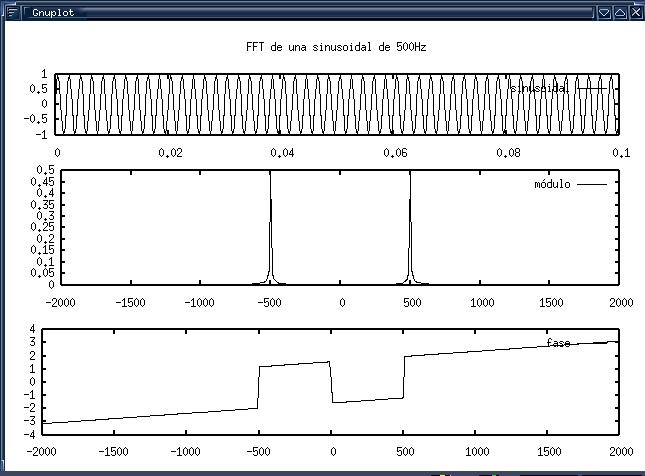
\includegraphics[width=0.8\textwidth]{imagenes/fftview1.m.eps}}
\subfigure[Ejemplo de FFT aplicado a una función escalón]{%
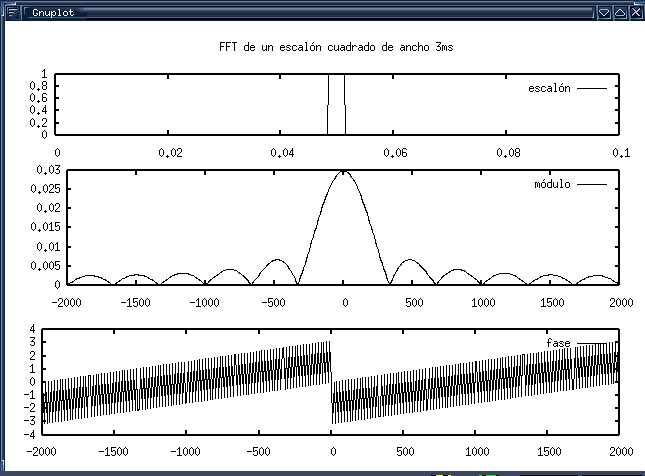
\includegraphics[width=0.8\textwidth]{imagenes/fftview2.m.eps}}
\end{figure}

% estaría bien poner un filtro de ejemplo, antes y después de pasar
% una señal por el.

\section{Tratamiento de imágenes}

\index{Octave!tratamiento de imágenes}

Por  último veamos  un  ejemplo  de cómo  se  pueden cargar,  realizar
modificaciones,  visualizar y  salvar imágenes  usando las  rutinas de
octave.  Con  esto  podremos  realizar muchas  operaciones  útiles  en
procesado, realzado y análisis de  imágenes, útiles en muchas áreas de
las ciencias.

En primer lugar suponemos sabido que una imagen se puede entender como
una matriz  donde cada punto tiene  un color diferente. Cada  punto se
llama {\em píxel}. Hay muchas  formas de representar pixeles, y octave
maneja tres de ellas, que son las siguientes:

\begin{description}

\item[escala de grises]  En una imagen en escala de  grises cada píxel
se  representa  por  un  valor de  punto  flotante  comprendido  entre
0,  que  significa  negro,  y  1, que  significa  blanco.  Por  tanto,
la  representación  de una  imagen  es  una  matriz llena  de  valores
comprendidos entre 0 y 1. En  este caso, un valor de 0.5 representaría
un color gris que tiene partes  iguales de blanco y negro mientras que
un valor de  0.2 representaría un color  que tiene 20\% de  negro y el
resto de blanco.

\item[color RGB] Cualquier  color en la naturaleza  se puede aproximar
(no es una  correspondencia exacta) como suma de  sus tres componentes
de color, a saber:  rojo (R, red), verde (G, green)  y azul (B, blue).
De esta forma, cada píxel de  una imagen en color se puede representar
como  un terna  de valores  de sus  tres componentes.  Por tanto,  una
imagen en formato  RGB son tres matrices del mismo  tamaño, donde cada
una almacena los valores de una componente.

\item[color  indexado]   Como  en  una  imagen   suele  haber  colores
repetidos,  esta representación  lista  por un  lado  los colores,  de
manera consecutiva y  sin repetirse, y por otro lado  los pixels, cuyo
color  se  almacena  buscando  el  valor en  la  tabla  de  colores  y
almacenando el índice correspondiente en el vector.

\end{description}

La  función  usada  para  representar imágenes  en  pantalla  es  {\tt
imshow()}. En  primer lugar  la usaremos  para representar  valores en
escala de grises. Vamos a probar creando una matriz que tenga variedad
de valores y presentándola. Veamos el ejemplo de uso de esta función:

\begin{verbatim}
octave:15> a=0:0.01:1;
octave:16> ma=a'*a;
octave:17> imshow(ma,2)
octave:18> imshow(ma,16)
octave:19> imshow(ma,256)
\end{verbatim}

\begin{figure}[htbp]
\centering
\subfigure[2 niveles]{%

\includegraphics[width=0.32\textwidth]{imagenes/image1a.m.eps}}
\subfigure[16 niveles]{%

\includegraphics[width=0.32\textwidth]{imagenes/image1b.m.eps}}
\subfigure[256 niveles]{%

\includegraphics[width=0.32\textwidth]{imagenes/image1c.m.eps}}
\caption[Gradiente visualizado a varios niveles de gris]%
{El gradiente anterior visualizado a varios niveles de gris}
\end{figure}

Observando la matriz  {\tt ma} observamos que todos  sus valores están
en el  rango $[0,1]$. Si  vemos su tamaño,  vemos que es  100x100. Las
diferentes  llamadas  a {\tt  imshow}  se  diferencian en  el  segundo
parámetro  que representa  el número  de colores  discretos en  el que
presentará la imagen continua. En el primer caso veremos solamente dos
colores, en la segunda 16 y en la tercera 256.

Probemos ahora  a trabajar con  una imagen  en color. La  función {\tt
loadimage()}  se  utiliza para  cargar  imágenes  de un  archivo.  Las
imágenes se devuelven en formato  indexado, donde {\tt c} representará
la matriz y {\tt cmap} representará los colores. Veamos el ejemplo:

\begin{verbatim}
octave:26> [c,cmap]=loadimage("tux.img");
octave:27> imshow(c,cmap)
\end{verbatim}

Como  verás, se  visualiza con  la misma  función. Ahora,  usemos esta
imagen como  base para  jugar un poco.  Primero, transformémosla  a un
formato  más  manejable. Empezaremos  pasándola  a  {\tt RGB}  con  la
función {\tt ind2rgb}  transforma la imagen de indexada  a RGB. Luego,
con {\tt imshow} la representaremos.

\begin{verbatim}
ctave:28> [r,g,b]=ind2rgb (c,cmap);
octave:29> imshow(r,g,b)
octave:30> imshow(g,r,b)
octave:31> imshow(b,g,r)
\end{verbatim}

\begin{figure}[htbp]
\centering
\subfigure[{\tt imshow(r,g,b)}]{%

\includegraphics[width=0.32\textwidth]{imagenes/image2a.m.eps}}
\subfigure[{\tt imshow(g,r,b)}]{%

\includegraphics[width=0.32\textwidth]{imagenes/image2b.m.eps}}
\subfigure[{\tt imshow(b,g,r)}]{%

\includegraphics[width=0.32\textwidth]{imagenes/image2c.m.eps}}
\caption[Imagen en color cambiando las componentes RGB]%
{Los colores de la imagen vienen representados por sus componentes
RGB. Si se invierten, los colores cambian.}
\end{figure}

Observamos  que  cada  canal  contiene sus  valores,  y  cambiando  el
orden hacemos  creer a  imshow que  los valores  son diferentes  y nos
muestra imágenes  con los colores trasladados.  Podemos probar también
sustituyendo las matrices {\tt r}, {\tt g}  o {\tt b} por unos o ceros
y  comprobar el  efecto de  quitar o  añadir canales.  El trabajo  con
imágenes RGB  es complejo, así  que usaremos  una imagen en  escala de
grises para seguir efectuando nuestras pruebas.

\begin{verbatim}
octave:32> g=ind2gray (c,cmap);
octave:35> imshow(g,2)
octave:36> imshow(g,4)
octave:37> imshow(g,16)
octave:65> imshow(g,256)
\end{verbatim}

\index{Octave!filtrado de imágenes}

Comenzaremos los análisis con  un filtrado/realzado. Estas operaciones
se realizan  barriendo todos  los píxels  de la  imagen y  creando una
nueva imagen  donde cada píxel  es una  ponderación de los  valores de
cada  píxel y  sus vecinos  según unas  matrices preestablecidos.  Las
matrices

\[
\begin{array}{ccc}
\frac{1}{5}\left( \begin{array}{ccc}
0 & 1 & 0\\
1 & 1 & 1\\
0 & 1 & 0
\end{array}\right)  & \left( \begin{array}{ccc}
0 & -1 & 0\\
-1 & 5 & -1\\
0 & -1 & 0
\end{array}\right)  & \left( \begin{array}{ccc}
0 & -1 & 0\\
-1 & 4 & -1\\
0 & -1 & 0
\end{array}\right) \\
\textrm{Filtro pasa-baja} & \textrm{Filtro pasa-alta} & \textrm{Detector de bordes}
\end{array}\]

Ahora veamos como  se aplicaría un filtro. Este filtro  es el primero,
que  genera una  imagen  donde  cada píxel  es  un  promedio entre  el
correspondiente en  la imagen original  y sus cuatro vecinos  por cada
lado.

\begin{verbatim}
octave:41> h=zeros(256,256);
octave:42> for i=2:255;
>             for j=2:255;
>                h(i,j)=(g(i,j)+g(i-1,j)+g(i+1,j)+ \
>                       g(i,j-1)+g(i,j+1))/5;
>             endfor;
>          endfor;
octave:43> imshow(g,256)
octave:44> imshow(h,256)
\end{verbatim}

Mostrando la imagen original y  retocada comprobamos que el efecto que
tiene es el de suavizar los bordes de la imagen, el de emborronarla.

Habrás notado que  has tenido que esperar un rato  (según la velocidad
de  tu  máquina)   durante  un  buen  rato  para   ver  el  resultado.
Este  procedimiento   es  optimizable  atendiendo  a   las  especiales
características de manejo  de matrices de octave. En vez  de hacer las
operaciones  elemento  a  elemento  con  sus  superiores,  inferiores,
izquierdo  y   derecho,  podemos  hacerlas   globalmente,  simplemente
trabajando con  las matrices  completas y operando  con ellas  con sus
desplazadas una posición hacia arriba,  abajo, izquierda y derecha. El
ejemplo esta aquí  y comprobarás que el resultado  es notablemente más
rápido.

\begin{verbatim}
octave:44> i=2:255;
octave:45> h=(g(i,i)+g(i-1,i)+g(i+1,i)+g(i,i-1)+g(i,i+1))/5;
octave:46> imshow(g,256)
octave:47> imshow(h,256)
\end{verbatim}

Comprobemos ahora los otros dos filtros. El siguiente filtro pasa-alta
se  implementaría así.  El resultado,  al contrario  que el  anterior,
acentúa los bordes en la  imagen, resultando los pequeños detalles más
destacados a simple vista.

\begin{verbatim}
octave:44> i=2:255;
octave:45> h=5*g(i,j)-g(i-1,j)-g(i+1,j)-g(i,j-1)-g(i,j+1);
octave:46> imshow(g,256)
octave:47> imshow(h,256)
\end{verbatim}

\begin{figure}[htbp]
\centering
\subfigure[Imagen original]{%

\includegraphics[width=0.32\textwidth]{imagenes/image3a.m.eps}}
\subfigure[Filtro pasa-baja]{%

\includegraphics[width=0.32\textwidth]{imagenes/image3b.m.eps}}
\subfigure[Filtro pasa-alta]{%

\includegraphics[width=0.32\textwidth]{imagenes/image3c.m.eps}}
\caption[Imagen tras aplicarle un filtro pasa-baja y pasa-alta]%
{Cuando aplicamos un filtro pasa-baja se suaviza la imagen y si 
aplicamos un pasa-alta, sus detalles se acentúan.}
\end{figure}

\index{Octave!detección de bordes}

Y por último, el  detector de bordes, que lo que  hace es presentar de
color blanco  las zonas que en  la imagen original tienen  cambios más
rápidos, mientras que las zonas  más homogéneas las presenta en negro.
Con esto, conseguimos detectar bordes acusados en la imagen.

\begin{verbatim}
octave:44> i=2:255;
octave:45> h=5*g(i,j)-g(i-1,j)-g(i+1,j)-g(i,j-1)-g(i,j+1);
octave:46> imshow(g,256)
octave:47> imshow(h,256)
\end{verbatim}

\begin{figura}{image4.m}{.8}
\caption{Imagen tras aplicar detector de bordes.}
\end{figura}
